Use the implicit Milne method to numerically solve

$$
u'(t) = 2(t + 1),\; u(1) = 3
$$

\begin{solution}\ \\\\
    \ \\
    For $f(t, U) = 2(t + 1)$, Milne's method on a uniform grid with spacing $k$ becomes:
    
    \begin{align*}
        u_{n+2} - u_n &= k \left[ \frac{2}{3}(t_n + 1) + \frac{8}{3}(t_{n+1} + 1) + \frac{2}{3}(t_{n+2} + 1) \right] \\
                      &= \frac{k}{3} \left[ (2t_n - 2k + 2) + (8t_n + 8) + (2t_n + 2k + 2) \right] \\
                      &= 4k(t_n + 4).
    \end{align*}
    
    We implement this in \texttt{problem\_2b.m} with \texttt{MATLAB} on the interval $t = [1, 5]$ with initial condition 
    $u(1) = 3$ and varying step sizes: \footnote{
        Note that the analytical solution to this ODE is given by $u(t) = t^2 + 2t$.
    }
    
    \begin{figure}[h]
        \centering
        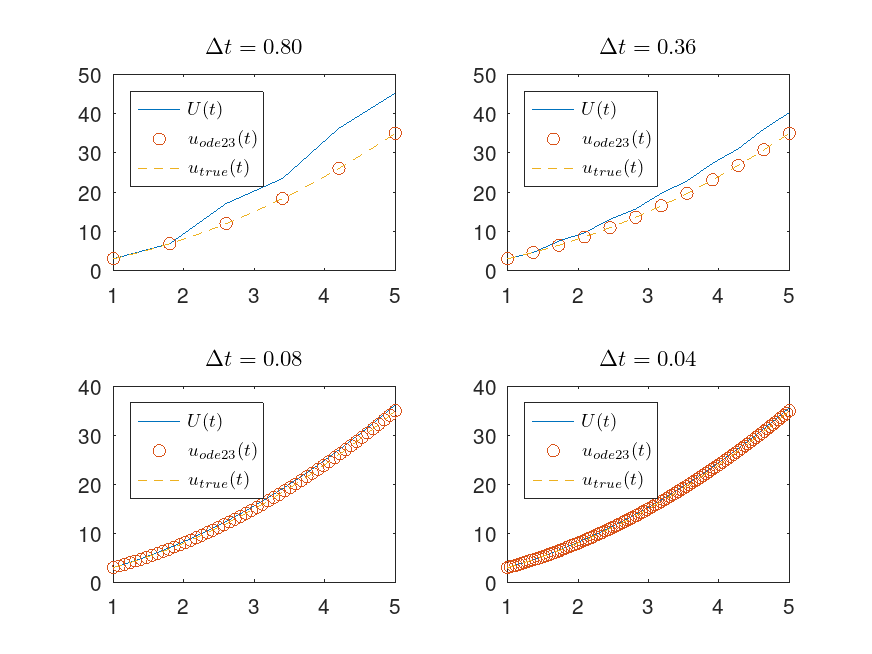
\includegraphics[width=0.85\textwidth]{problem_2b_solution.png}
        \caption[problem2b_solution]{Implicit Milne method solution to $u' = 2(t+1),\; u(1) = 3$}
    \end{figure}
\end{solution}